\documentclass[a4paper,11pt,twocolumn]{article}

\usepackage{fullpage}
\usepackage[hidelinks]{hyperref}
\usepackage{graphicx}
\usepackage{float}
\usepackage[english]{babel}

\title{\textsc{Team Classified} \\ \small{Sberbank Russian Housing
Market\footnote{https://www.kaggle.com/c/sberbank-russian-housing-market}}}
\author{Jordi Beernink \and Roel Bouman \and Jeffrey Luppes \and Gerdriaan Mulder \and Thijs Werrij}

\begin{document}
\maketitle

\section{Introduction}
This report details the work done on the Sberbank Housing Competition set by the
Classified Team. The competition ran roughly from the start of May until the end
of June. Thus, this report was written two weeks before the final deadline and
may not reflect the final standings in the competition.

\section{Problem description}
Sberbank, a state owned and largest bank in Russia. Sberbank is involved in
financing and brokering deals in the Russian realty market and thus heavily
relies on models to predict the value of property. Although the Russian house
market remains fairly stable, Russia's economy relies on natural resources and
is therefore often subjected to volatile changes. This makes predicting property
value and correcting for the economy a non-trivial task.

The goal of the Kaggle competition is to predict realty prices. A feature-rich
dataset based on data from 30000 properties (e.g. apartments) from 2011 until
2015 is available for training, and a separate split from 2015 until 2016 is
available for testing. The true prices of the test set are not known, and the
public leaderboard is based on 35\% of the test data. Additionally, a data set
containing macro-economic data is available which also goes into high detail.

The metric used for the leaderboard is the \emph{Root Mean Squared
Logarithmic Error} (\mbox{RMSLE}). Submissions are limited to five per day.

\section{Approach}

\subsection{Early exploratory work and visualization}
Some exploratory work was done in Apache
Spark\footnote{\url{https://rubigdata.github.io/bigdata-blog-2017-jeffluppes/2017/05/04/Give-me-a-spark/}},
Python plots and with use of the leaflet JavaScript library for plotting data on
a map. This served to get a good feel for the data as well as early
identification of outliers and missing data.

\subsection{Exploratory analysis}
The training data was supplied as numerical and categorical data. In order to
work with e.g. a Random Forest Regressor (sklearn) this needed to be one-hot
encoded. For validation purposes, the training set was split in a new training
set containing all entries before 2015, and a validation set consisting of all
entries in 2015. Using some internal validation, various methods were
preliminarily tested. These methods include Linear Regression, Random Forests,
AdaBoost, KNN, XGBoost, Deep Learning and Stochastic Gradient Descent. These
methods are easy to use, readily available, and have been proven to work
decently . It quickly became clear that Extreme Gradient Boosting, or XGBoost,
outperformed all other methods with a significant margin. It is hypothesized
that XGBoost outperforms other methods by its inherent ensemble property, being
able to robustly handle different categories of data. The boosting of weak
learners might emphasize the variables that are useful for prediction, whilst
de-emphasizing variables indicating fraud.  There was little correlation between
internal validation, and validation using the Kaggle submissions platform. It is
likely that this is caused by the presence of fraud in data, which is
influential in validation, and may be present in a lesser degree in the test
set. Another explanation might be that there are some discrepancies in the
time-price trend correction, which causes an offset in the evaluation error.
Various forms of validation, including K-fold Cross Validation, provided no
improvement, greatly decreasing the usefulness of validation. The dataset was
far from complete, and many entries were missing data. It was particularly
viable to improve the performance by focusing on pre-processing.


\subsection{Imputing data}
Various methods of imputing, such as KNN and SVD-based methods, have been tested
or tried. Matrix Factorization methods, like those used in the famous Netflix
competition, were not readily available to be used, and were too costly to
develop internally. KNN and SVD based methods rely on the construction of large
matrices of \emph{sample-x-sample} size, which were unfeasible, as they have
estimated sizes of over 90GB. More memory-efficient implementations were again
not available. Simpler methods, like using mean, modus or median offered no
improvement over not replacing the NaN values in the data. Not replacing the NaN
values means some numerical variables can not be used for prediction. For
categorical variables, NaN values are treated as a separate category.

\subsection{Regression using XGBoost and Keras}
In the early part of the competition, single models using XGBoost performed
reasonably well, yielding results in the top 20\%. Deep Learning methods using
Keras were not able to compete, and, regardless of network complexity, did not
come close to the performance of single XGBoost models. Deep Learning might
suffer more from a lack of appropriate regularization and an overemphasis of
non-important features. This might perhaps be alleviated with more
experimentation with other activation layers or a better batch selection
procedure.

Nearing the end of the competition and near the project deadline, a modestly
successful kernel was published. This kernel was an ensemble of three XGBoost
models, which, when combined, were able to hit top 5\% at the date of
publication. The bulk of further work was based on these models, being mostly
based on ensemble weighting tweaking. Using linear regression to optimize
ensemble weighting was briefly tested, but was hindered by the little
correlation between validation and testing sets. A graphical representation of
the final model, including the XGBoost parameter settings and other weightings
can be found in appendix~\ref{app:final}.

\section{Results}
The results of some key submissions and models are illustrated in
table~\ref{tbl:xval}. These
may not reflect the final standings. For each implementation details are listed
regarding the error returned by Kaggle. A lower score indicates a better
performing model. These results are discussed in depth in the next section.

\begin{table*}[ht]
    \centering
    \begin{tabular}{| p{.25\textwidth} | p{.3\textwidth} | p{.1\textwidth} |
    p{.2\textwidth}|}
    \hline
    \textbf{Classifier} & \textbf{Method} & \textbf{RMSLE} & \textbf{Kaggle Rank
    (of~3077)} \\
    \hline
    XGBoost & Ensemble with 3 models, readjustment of submission & 0.31038 & 146 \\
    \hline
    XGBoost & Ensemble with 3 models & 0.31062 & 266 \\
    \hline
    XGBoost & Single & 0.32575 & 1856 \\
    \hline
    Gradientboosting Regressor & Complete dataset, only 2015 & 0.41384 & 2767 \\
    \hline
    Deep Learning & Dense and Dropout & 0.46745 & 2870 \\
    \hline
    Linear Regression & Complete dataset, only 2015 & 0.49689 & 2897 \\
    \hline
    Decision Tree & Complete dataset, only 2015 & 0.58460 & 3020 \\
    \hline
    SGD Regressor & Naive & 0.59560 & 3021 \\
    \hline
    Benchmark Submission & Naive XGBoost & 0.67333 & 3034 \\
    \hline
    Random Forests & Removing outliers, only 2015 & 0.75239 & 3040 \\
    \hline
    k-Nearest Neighbours & $k = 6$, removing outliers, only 2015 & 0.93122 &
    2050 \\
    \hline
    Random Forest & Naive & 6.12138 & 3072 \\
    \hline
    \end{tabular}
\caption{Overview of key submissions with their models, result and rank}
\label{tbl:xval}
\end{table*}

\section{Discussion}
The ensemble of three XGBoost models performed better than any other method,
including previous XGBoost models individually. Early on in the completion these
performed with modest success, as they ended up in the middle of the segment.

Performance of many classic regression methods was poor. The high complexity and
sparsity of the data set particularly difficult for these models, as there are
many patterns not identified by linear methods. Still, it was thought these
could be included in the ensemble but intermediate results were not affirming
any potential in this approach.

The best method was an XGBoost Ensemble based on a published kernel by Kaggle
user and Econometrist Andy
Harless\footnote{\url{https://www.kaggle.com/aharless/latest-iteration-in-this-silly-game}},
which included work from other Kaggle contributors. This model was improved
upon, and outperformed the original Kernel which on its own quickly saw wide
adaption within the community.

Sadly, the Keras approach (‘Deep Learning’ in table~\ref{tbl:xval}), a 10-layer deep neural
network could not compete with the success of XGBoost implementations

Unlike the first competition Kaggle kernels were used with good success. Equally
much as starting point, inspiration for our own approaches, and keeping a close
eye on what the community was coming up with. Some of the code written was also
published on Kaggle in the form of Kernels.

As stated and elaborated earlier, the in-house evaluation method based on the
training data proved to have no correlation to success on the leaderboard. This
was the experience of other Kaggle users as well, as there are a lot of
disgruntled posts on the forum.

At the moment of writing (June 19th, 2017) the highest score achieved was
0.31038 with (currently) the rank of 134/3175. This places us in the top
four/five percent. The all-time highest placement was rank 49 (top 1.5\%) with
0.31062 obtained on June 5, which was gradually lost over the next days.
Overall, the team made over 50 submissions. If the competition would end today,
we would be awarded silver.

\section{Criticism}
The competition is not without flaws. The test set being much different (both in
balance, and quality) than the training data that was given made evaluation of
candidate submissions hard to do. Without a proper method of model validation we
were in the dark. A lot of data was missing and fraud was suspected in a
significant amount of
objects\footnote{\url{https://www.kaggle.com/c/sberbank-russian-housing-market/discussion/32608}}.
Some major issues like the distance from schools, hospitals and such were
actually based on the distance from/to the housing agencies instead of the
properties themselves, were only published late in the competition.

\newpage

\onecolumn
\section{Individual contributions}
We started our project with an exploration of the data, in which we all analyzed
the data, generated images and reported our findings in our group meetings. This
free-form allowed us to explore a lot of ideas. After this we decided how we
would tackle the problem: Jordi and Roel would do pre-processing, Gerdriaan and
Thijs would try different classifiers and see what works well and Jeffrey would
look at constructing an ensemble in addition to standard regression models.

Gerdriaan tested stochastic gradient descent (SGD) and Thijs looked at Keras
Deep Neural Networks, both of which had results that did not look promising
enough to improve on. After discovering the Magic Numbers kernel on Kaggle,
mostly Jordi, Roel and Jeffrey worked at improving this script and making
submissions.

Notes taken at our meetings were written by Jordi. The flash talk was presented
by Jeffrey. To finish the project, we wrote the report together, with editing in
the hands of Jeffrey. Gerdriaan worked on the code delivery, and Thijs and
Jeffrey made and presented the final presentation.

\clearpage

\appendix
\section{The final ensemble method}
\label{app:final}

\begin{figure}[H]
\centering
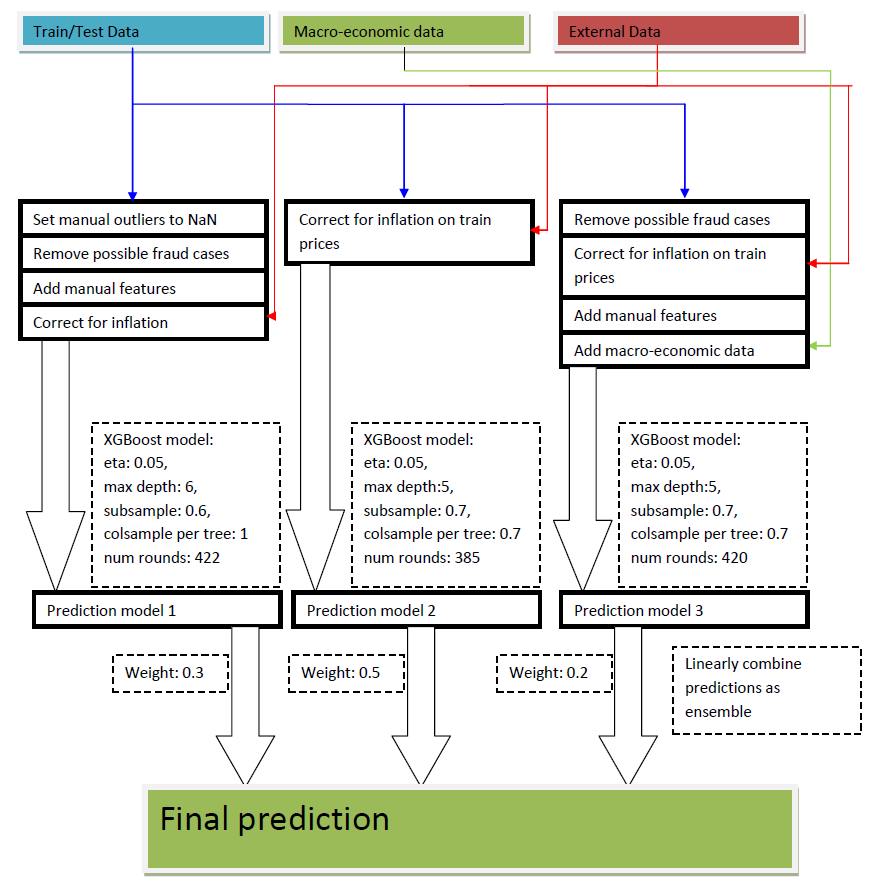
\includegraphics[width=\textwidth]{ensemble.png}
\label{fig:ens}
\end{figure}

The train, test and macro-economic data can be found in train.csv, test.csv and
macro.csv respectively.

Manual outlier detection consisted of detection of data that was incorrect based
on simple logic heuristics. This covers cases such as square meters of the
kitchen and living room not adding up to the total mentioned under that of the
kitchen and living room together, as well as possible typo's in for example room
number, such as 100 square meter apartments contained 126 rooms.

Some further fraud detection was done by removing extremely high prices from the
training set. A manual selection was made by some Kagglers, based on apartments
selling for 2-5 the price of regular (identical) apartments.


\end{document}
